\documentclass[main.tex]{subfiles}
\begin{document}

\marginpar{Wednesday\\ 2020-11-25, \\ compiled \\ \today}

We wanted to estimate the magnetic field \(B\) and characteristic age \(\tau _c\) of the NS: we have found that \(B_P \propto \sqrt{P \dot{P}}\) and \(\tau _c \propto P / \dot{P}\).

Now we will define the \textbf{braking index}: recall that the evolution of the angular velocity can be written as \(\dot{\Omega} = - k \Omega^3\). 
This can be generalized to a law of the type \(\dot{\Omega} = -k \Omega^{n}\); the spin-down due to the emission of GWs is similarly written with \(n = 6\). 

Taking the derivative of this law, we find 
%
\begin{align}
\ddot{\Omega} &= - kn \dot{\Omega} \Omega^{n-1}  \\
&= \frac{n}{\Omega } \dot{\Omega} (-k \Omega^{n}) = n \frac{\dot{\Omega}^2}{\Omega }   \\
n &= \frac{\ddot{\Omega} \Omega }{\dot{\Omega}^2}
\,.
\end{align}

By measuring \(\Omega \), \(\dot{\Omega}\) and \(\ddot{\Omega}\) we can estimate \(n\), which will allow us to find the braking index \(n\).
However, as the order of the derivative increases the difficulty of the measurement increases. The index \(n\) is known for around 10 NSs, and it was measured to be \(n < 3\), which is evidence against magnetorotational losses as the main cause of the spin-down. 

We make a plot, with  \(\log P\) on the \(x\) axis and \(\log \dot{P}\) on the \(y\) axis: this is the \(P-\dot{P}\) diagram.
We can scatter-plot known NSs in it: see figure \ref{fig:p-pdot-diagram}.

\begin{figure}[ht]
\centering
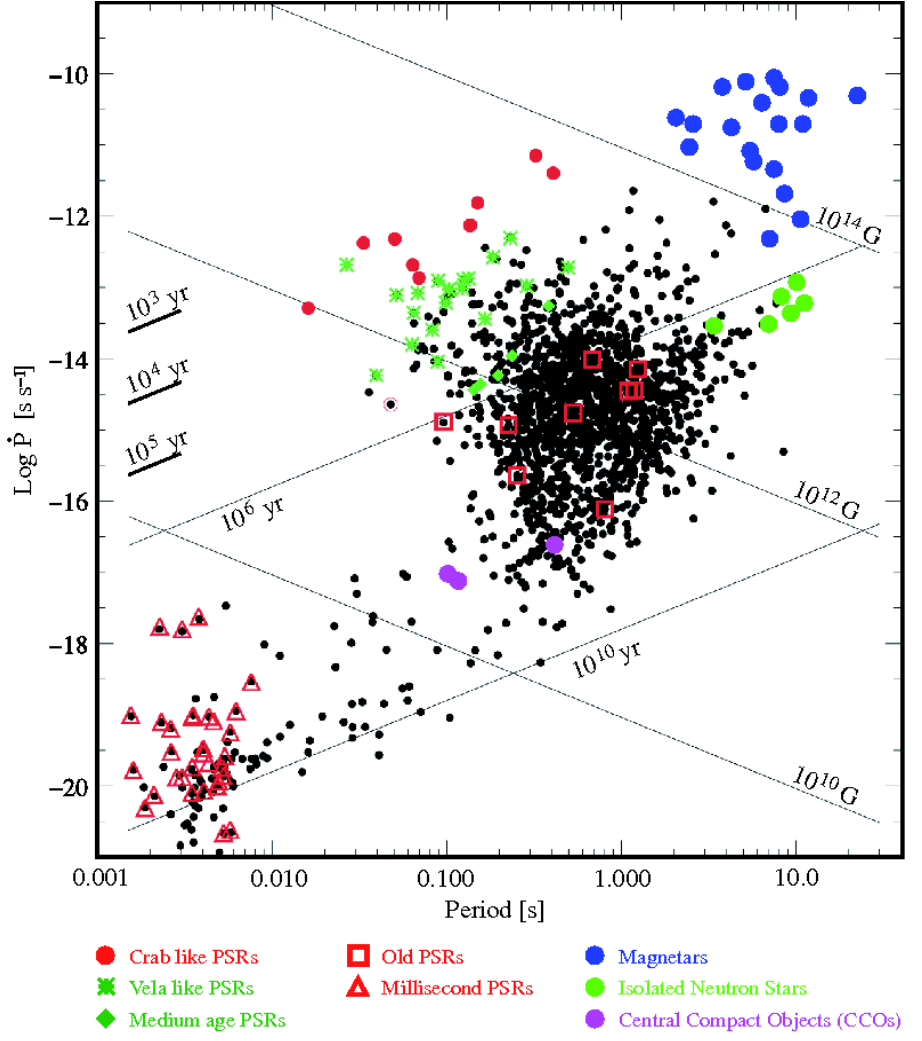
\includegraphics[width=.8\textwidth]{figures/p-pdot-diagram}
\caption{An example \(P-\dot{P}\) diagram from \textcite[]{beckerAutonomousSpacecraftNavigation2013}.}
\label{fig:p-pdot-diagram}
\end{figure}

Equal-\(B_p\) lines and equal-\(\tau _c\) lines can be drawn: 
the first are in the form \(\log P = - \log \dot{P} + k\), the second are in the form \(\log P = \log \dot{P} + k\). 
We can track the motion of NSs through this diagram: they will move down and to the right as they evolve, with a slope of \(2 - n\), since 
%
\begin{align}
\dv{t}( \frac{1}{P}) \propto - \frac{1}{P^{n}} \implies \dot{P} \propto P^{2-n}
\,.
\end{align} 

\section{Interior structure of NSs}

Are they actually made of neutrons? Mostly, yes, but not exclusively.

A free neutron will \(\beta \)-decay:  
%
\begin{align}
\ce{n} \to e^{-} + \ce{p} + \overline{\nu}
\,
\end{align}
%
within around \SI{15}{min}. Neutrons are also formed through inverse \(\beta \)-decay (also called electron capture): 
%
\begin{align}
e^{-} + \ce{p} \to \ce{n} + \nu 
\,.
\end{align}

This process, however, is endothermic: \(m_e + m_p < m_n \). 
Specifically, \(Q = (m_n - m_p)c^2 \approx 2.54 m_e c^2\approx \SI{1.3}{MeV}\) is the energy the electron must have in order to achieve the reaction. 

The thermal energy is definitely not that high inside a NS!
In order to describe what goes on, we will make some assumptions:
\begin{enumerate}
    \item the interior is only made of neutrons, protons and electrons (the \(npe\) model) (this is not really true, but it will allow us to illustrate the point);
    \item the number densities of these species are similar: \(n_e \approx n_p \approx n_n\). 
\end{enumerate}

Matter inside a neutron star is highly degenerate: the energy of each electron is much smaller than the Fermi energy.
The Fermi energy can be written as \(E_F \approx m_e c^2 \sqrt{1 + x_F^2}\), where \(x_F = p_F / m_ec\), and 
%
\begin{align}
p_F = \sqrt[3]{\frac{3 h^3 n_e}{8 \pi }}
\,.
\end{align}

Therefore, 
%
\begin{align}
x_F = \sqrt[3]{\frac{3 h^3 n_e}{8 \pi }} \frac{1}{m_e c}
\approx \num{e-2} \sqrt[3]{\frac{\rho}{\mu }}
\,.
\end{align}

If we want the electrons to be relativistic, we require \(x_F \gtrsim 1\), which means \(\rho / \mu _e \gtrsim \SI{e6}{g / cm^3}\). 

If the Fermi energy is as high as the \(Q\)-value of the reaction, \(E_F \gtrsim \num{2.54} m_e c^2\), then we must have 
%
\begin{align}
\sqrt{1 + x_F^2} \gtrsim \num{2.54} \implies x_F \gtrsim \num{2.3}
\,,
\end{align}
%
which can be solved in terms of the rest mass matter density: we get 
%
\begin{align}
\rho \gtrsim \SI{1.7e7}{g / cm^3} \times \mu _e
\,,
\end{align}
%
which is high in absolute terms, but rather low for a NS, since they typically will have densities several orders of magnitude higher. 

At these densities, not only electrons, but protons and neutrons are degenerate as well, however these more massive particles are not relativistic. 
In fact, \(x_F \propto n / m\) holds across particle species: protons and neutrons will have \(x_F^{(p, n)} \sim x_F^{(e)} / 2000 \), since they are \(\sim 2000\) times more massive. 

The densities needed for the neutrons and protons to be relativistic might be achieved in the very core of the star, but they are typically not. 

So, the electrons are relativistic and the reaction can happen back and forth at equilibrium: this means that we can equate their chemical potentials, 
%
\begin{align}
\mu _p + \mu _e = \mu _n (+ \mu _\nu )
\,,
\end{align}
%
where the neutrinos can be neglected since they generally fly away after a reaction, unable to interact further. 
Under complete degeneracy we have \(\mu = E_F\). 
Then, we can write 
%   
\begin{align}
m_p c^2 \sqrt{1 + x_p^2} +
m_e c^2 \sqrt{1 + x_e^2} =
m_n c^2 \sqrt{1 + x_n^2} 
\,,
\end{align}
%
but by charge neutrality we must have \(n_e = n_p\).
This is to be complemented with \(n \propto p_F^3\) and \(x = p_F / mc\): thus, \(x_e / x_p = m_p / m_e\).

Working through the algebra,\footnote{The passages to follow are: eliminate \(x_e\) in the previous equation with the relation \(x_e / x_p = m_p / m_e\), approximate \(\sqrt{1 + x^2}\) as \(x\) for electrons and as \(1 + x^2/2\) for protons and neutrons (thus assuming that they are nonrelativistic); solve for \(x_n / x_p\).}  we find 
%
\begin{align}
R_{np} = \frac{n_n}{n_p} = x_n^3 \qty[
    \frac{4 (1 + x_n^2)}{x_n^4 + \frac{4 Q x_n^3}{m_n} + 4\frac{(Q^2 -m_e^2)}{m_n^2}} 
]^{3/2}
= \frac{x_n^3}{x_p^3}
\,.
\end{align}

This is plotted on a log-log scale as a function of \(x_n\) in figure \ref{fig:neutron-proton-ratio}.

The density is given by 
%
\begin{align}
\rho &= m_e n_e + m_n n_n + m_p n_p \approx m (n_p + n_n)  
\marginnote{We define \(m = m_n \approx m_p\).}
\\
&\approx m \frac{8 \pi }{3} \qty(\frac{mc}{h})^3
\qty[x_p^3 + x_n^3]  \\
&= m \frac{8 \pi }{3} \qty(\frac{mc}{h})^3
x_n^3 \qty[ \frac{1}{R_{np} (x_n)} + 1]
\,.
\end{align}
%

This yields a parametric expression for \(R_{np}\) in terms of \(\rho \); if \(\rho \) is very small then \(n_n \ll n_p\), approaching \(n_n \sim 0\), around \(\rho \approx \SI{e12}{g / cm^3}\) there is a maximum of \(R_{np}\approx \num{e4}\), and it seems to approach \(R_{np} \sim 10 \) asymptotically. It is shown in figure \ref{fig:neutron-proton-ratio-density}.  

Taking the limit of the expression for  \(\rho \) as \(n_n \to 0\) we find 
%
\begin{align}
\rho &\approx \frac{m 8 \pi }{3} \qty(\frac{mc}{h})^3 \qty[ \frac{Q^2 - m_e^2}{m^2}]^{3/2}  \\
&\approx \frac{8 \pi m}{3} \qty( \frac{c}{h}\sqrt{Q^2 - m_e^2})^3 
\,.
\end{align}

This is around \SI{1.2e7}{g / cm^3}. It is expected, since below this density there will be no neutrons anymore. 
If we plot \(\rho (x_n)\), we see a plateau until about \(x_n \sim \num{e-2}\), after which we start to see \(\rho \propto x_n^3\).

\end{document}
